\chapter{Аналитический раздел}

В данном разделе проводится анализ существующих ЭБС и способов хранения данных, а также формализуются задача, структура хранимых данных и требования к системе.
\section{Обзор существующих решений}

\subsection{ЭБC <<Лань>>}
ЭБC <<Лань>> – электронно-библиотечная система, предоставляющая студентам, аспирантам и преподавателям подключенных библиотек доступ к чтению электронных версий книг, журналов. Для поиска информационных ресурсов организован гибкий поиск по различным фильтрам. Система не предоставляет возможности получения бумажных книг, а значит и интеграции в обычные библиотеки. 

\subsection{Московская ЭБС}
Московская ЭБС предоставляет возможность просмотра доступных книг во всех библиотеках Москвы, при этом функционал фильтрации довольно ограниченный. Система не предоставляет возможности онлайн доступа к информационным ресурсам и не поддерживает добавление библиотек, находящихся в других городах. 

\subsection{eLibrary}
eLibrary -- научная электронная библиотека, крупнейший российский ин- формационно-аналитический портал в области науки, технологии, медицины и образования, предоставляющий возможность разнообразной фильтрации и поиска. Система работает только с электронными ресурсами. Кроме того, система ориентирована только на научные труды, статьи и рефераты.

\subsection{Сравнение существующих решений}
\begin{table} [h!]
	\caption{Сравнительная таблица существующих решений}
	\begin{center}
	\begin{tabular}{|c c c c|}
    \hline
            & Возможность & Возможность& Возможность \\
     ЭБС       & использования & разнообразной& использования \\
           & в обычных & фильтрации & большой  \\
           & библиотеках &  & аудиторией  \\
    \hline
    Лань     & - & + & + \\
    \hline
    ЭБС & +& -& -  \\
    Москвы & & &   \\
    \hline
    eLibrary & - & + & +  \\
    \hline
	\end{tabular}
	\end{center}
\end{table}

На основе анализа существующих решений было выяснено, что в сети Интернет есть много ресурсов, позволяющих получить доступ к книгам в электронном виде. Такие сервисы предлагают возможность разнообразной фильтрации, однако они могут быть использованы исключительно в онлайн-режиме. Возможность интеграции в реальные библиотеки они не предусматривают. С другой стороны, во многих городах России есть системы, позволяющие записаться в библиотеки города или посмотреть наличие книг в них. Недостатком таких систем является то, что они не предоставляют возможности гибко фильтровать книги и то, что в разных городах (а иногда и в разных сетях библиотек города) системы разные. 

\section{Формализация задачи}
Требуется разработать электронную библиотечную систему, которая позволит читателям получать информацию о доступных книгах в разных библиотеках, а также информацию о ранее взятых книгах, библиотекарям -- выдавать и принимать книги, а администраторам библиотечной системы -- редактировать информацию о книгах и библиотеках.

Таким образом, выделяются 3 роли: читатель, библиотекарь, администратор.

Взаимодействие с продуктом происходит по схеме, представленной на рисунке \ref{fig:usecase}.

\begin{figure}[H]
	\centering
	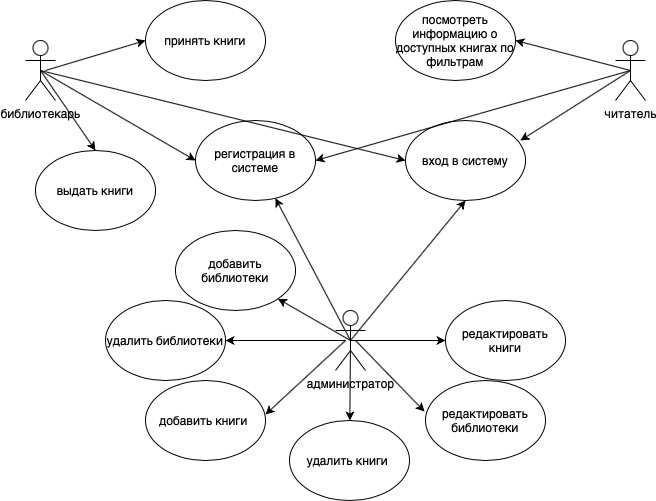
\includegraphics[width = \linewidth]{img/use-case.jpg}
	\caption{Use-case диаграмма}
	\label{fig:usecase}
\end{figure}

\section{\label{subd}Базы данных и структура хранимых данных}

В задаче разработки электронной библиотечной системы важную роль играет выбор модели хранения данных. Наиболее общим подходом к хранению данных является использование баз данных \cite{bib:1}. Для управления базами используется системы управления базами данных -- СУБД \cite{bib:2}. Система управления базами данных -- это совокупность программных и лингвистических средств общего или специального назначения, обеспечивающих управление созданием и использованием баз данных.
\newpage
Базы данных по способу хранения можно классифицировать следующим образом:
\begin{enumerate}
    \item  строковые базы данных;
    \item  колоночные базы данных.
\end{enumerate}

\noindent\textbf{Строковые базы данных}

Строковыми базами данных называются базы данных, данные в которых хранятся построчно. Базы данных этого типа применяются в системах, для которых характерно наличие большого количества коротких транзакций вставки, удаления, изменения. Важным показателем таких систем является их отзывчивость, то есть запросы должны обрабатываться быстро. 


\noindent\textbf{Колоночные базы данных}

Колоночными базами данных называются базы данных, данные в которых хранятся по столбцам. Базы данных этого типа применяются в системах, для которых характерно небольшое количество транзакций, однако при этом запросы могут быть достаточно сложными. 

\subsection{Выбор модели хранения данных}
Для реализации библиотечной системы было решено использовать построчное хранение данных, поскольку:
\begin{itemize}
	\item предполагается большое количество коротких транзакций;
	\item предполагается высокий уровень отзывчивости системы;
	\item не предполагается выполнение сложных аналитических запросов.
\end{itemize}

\subsection{Формализация структуры хранимых данных}
Для создания базы данных, хранящей библиотечную систему, выделены слудующие сущности предметной области: книга, экземпляр книги, библиотека, аккаунт, администратор, библиотекарь, читатель.

На рисунке \ref{fig:er} представлена диаграмма сущность-связь для данной задачи.

\begin{figure}[H]
	\centering
	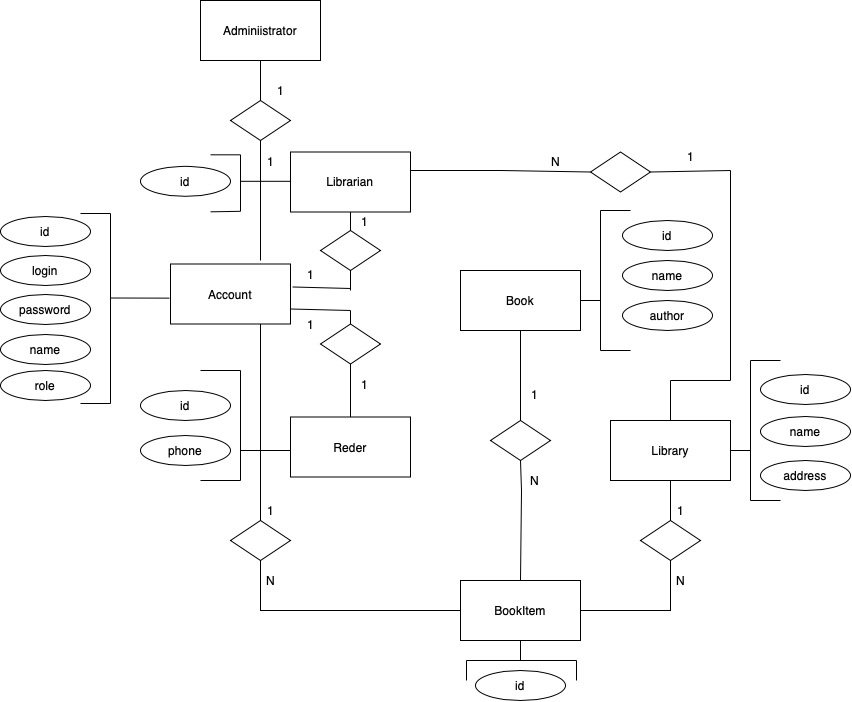
\includegraphics[width = \linewidth]{img/er_db.jpg}
	\caption{Диаграмма сущность-связь}
	\label{fig:er}
\end{figure}
\section*{Вывод}
\addcontentsline{toc}{section}{Вывод}

В данном разделе был проведён анализ существующих ЭБС и способов хранения данных. Было решено использовать строковую базу данных. Кроме того, были формализованы задача, структура хранимых данных и требования к системе.

